\section{Problem Set 8}

\subsection{Finalizing Navigation Methods}

We implemented our Kalman filter after completing the set-up work from last week. For our ground truth, we used the 2 body propagator with J2 effects that we developed early in the course. We then corrupted the ground truth with guassian noise (of zero mean and reasonable standard deviation) to simulate sensor measurements for the spacecraft. As discussed last week, we include 4 methods of sensing - relative position and velocity, and absolute position and velocity.

Our initial state estimate is set to the initial position of the simulation, while our initial covariance is set to the identity matrix. Similarly, we initially set Q and R to be identity matrices as well, and then tuned them to get reasonable filter results.

Our filter ended up working very well. In the graphs below, we plot the truth state from the 2 body propogator, next to the estimated state from the kalman filter. The additional plots describe the error and quality of the filter. The code for the filter lives in the appendix.

\begin{figure}[H]
    \centering
    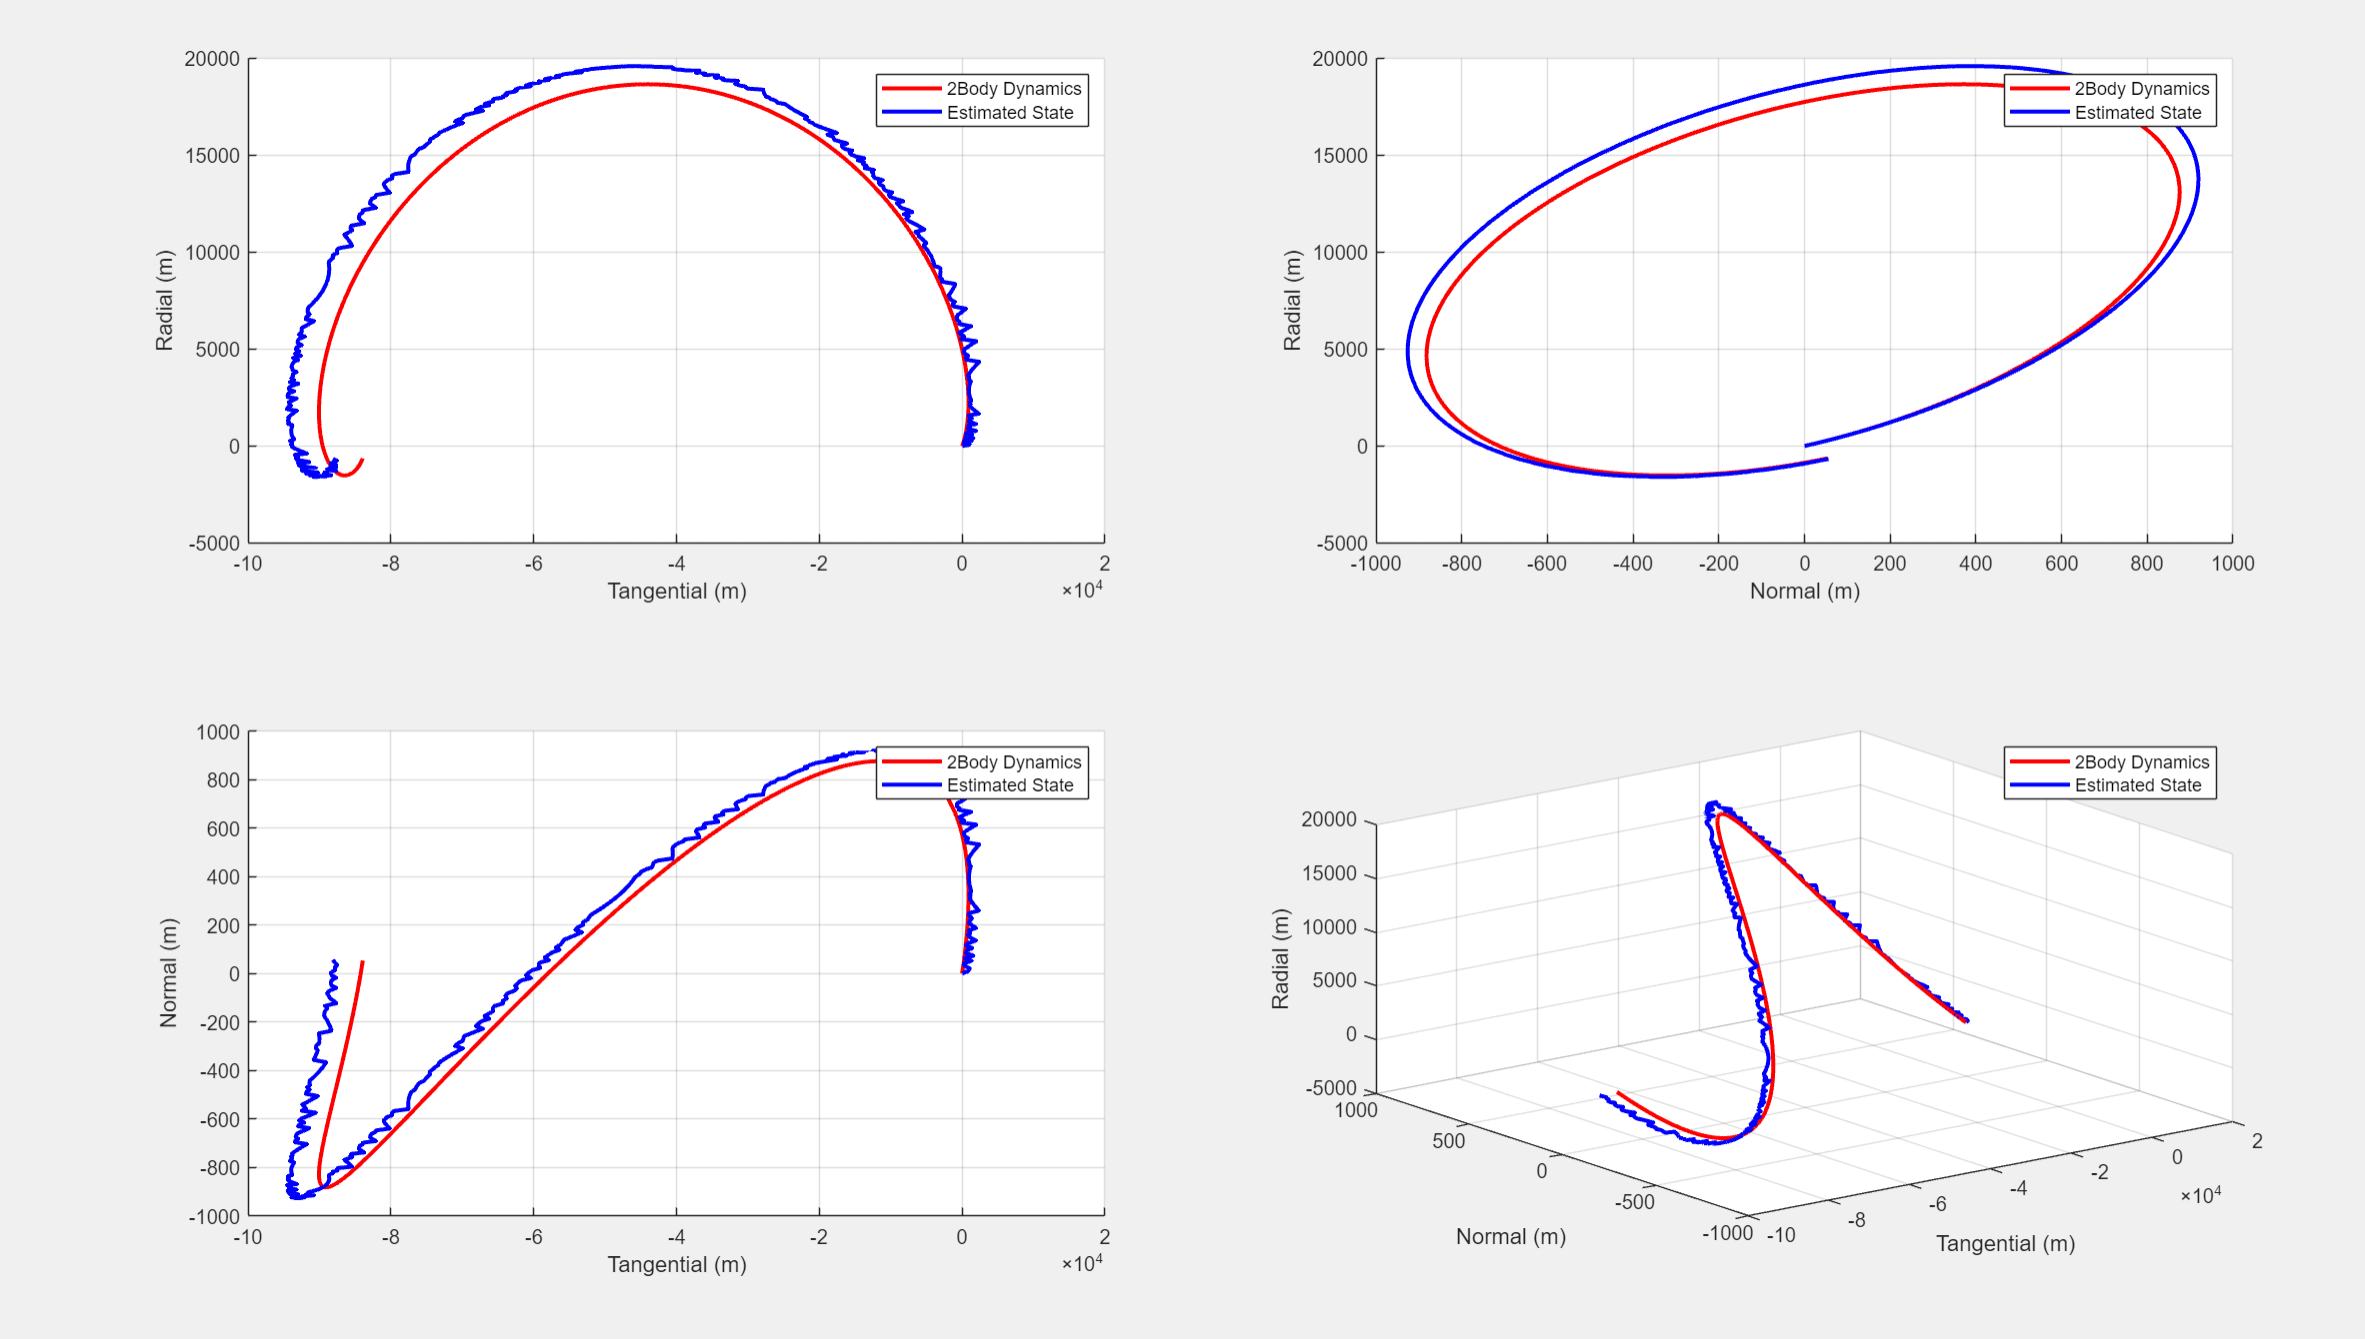
\includegraphics[width=0.7\textwidth]{PS8/Figures/position.png}
    \caption{Estimated Position}
    \label{fig:hcw_velocity}
\end{figure}

\begin{figure}[H]
    \centering
    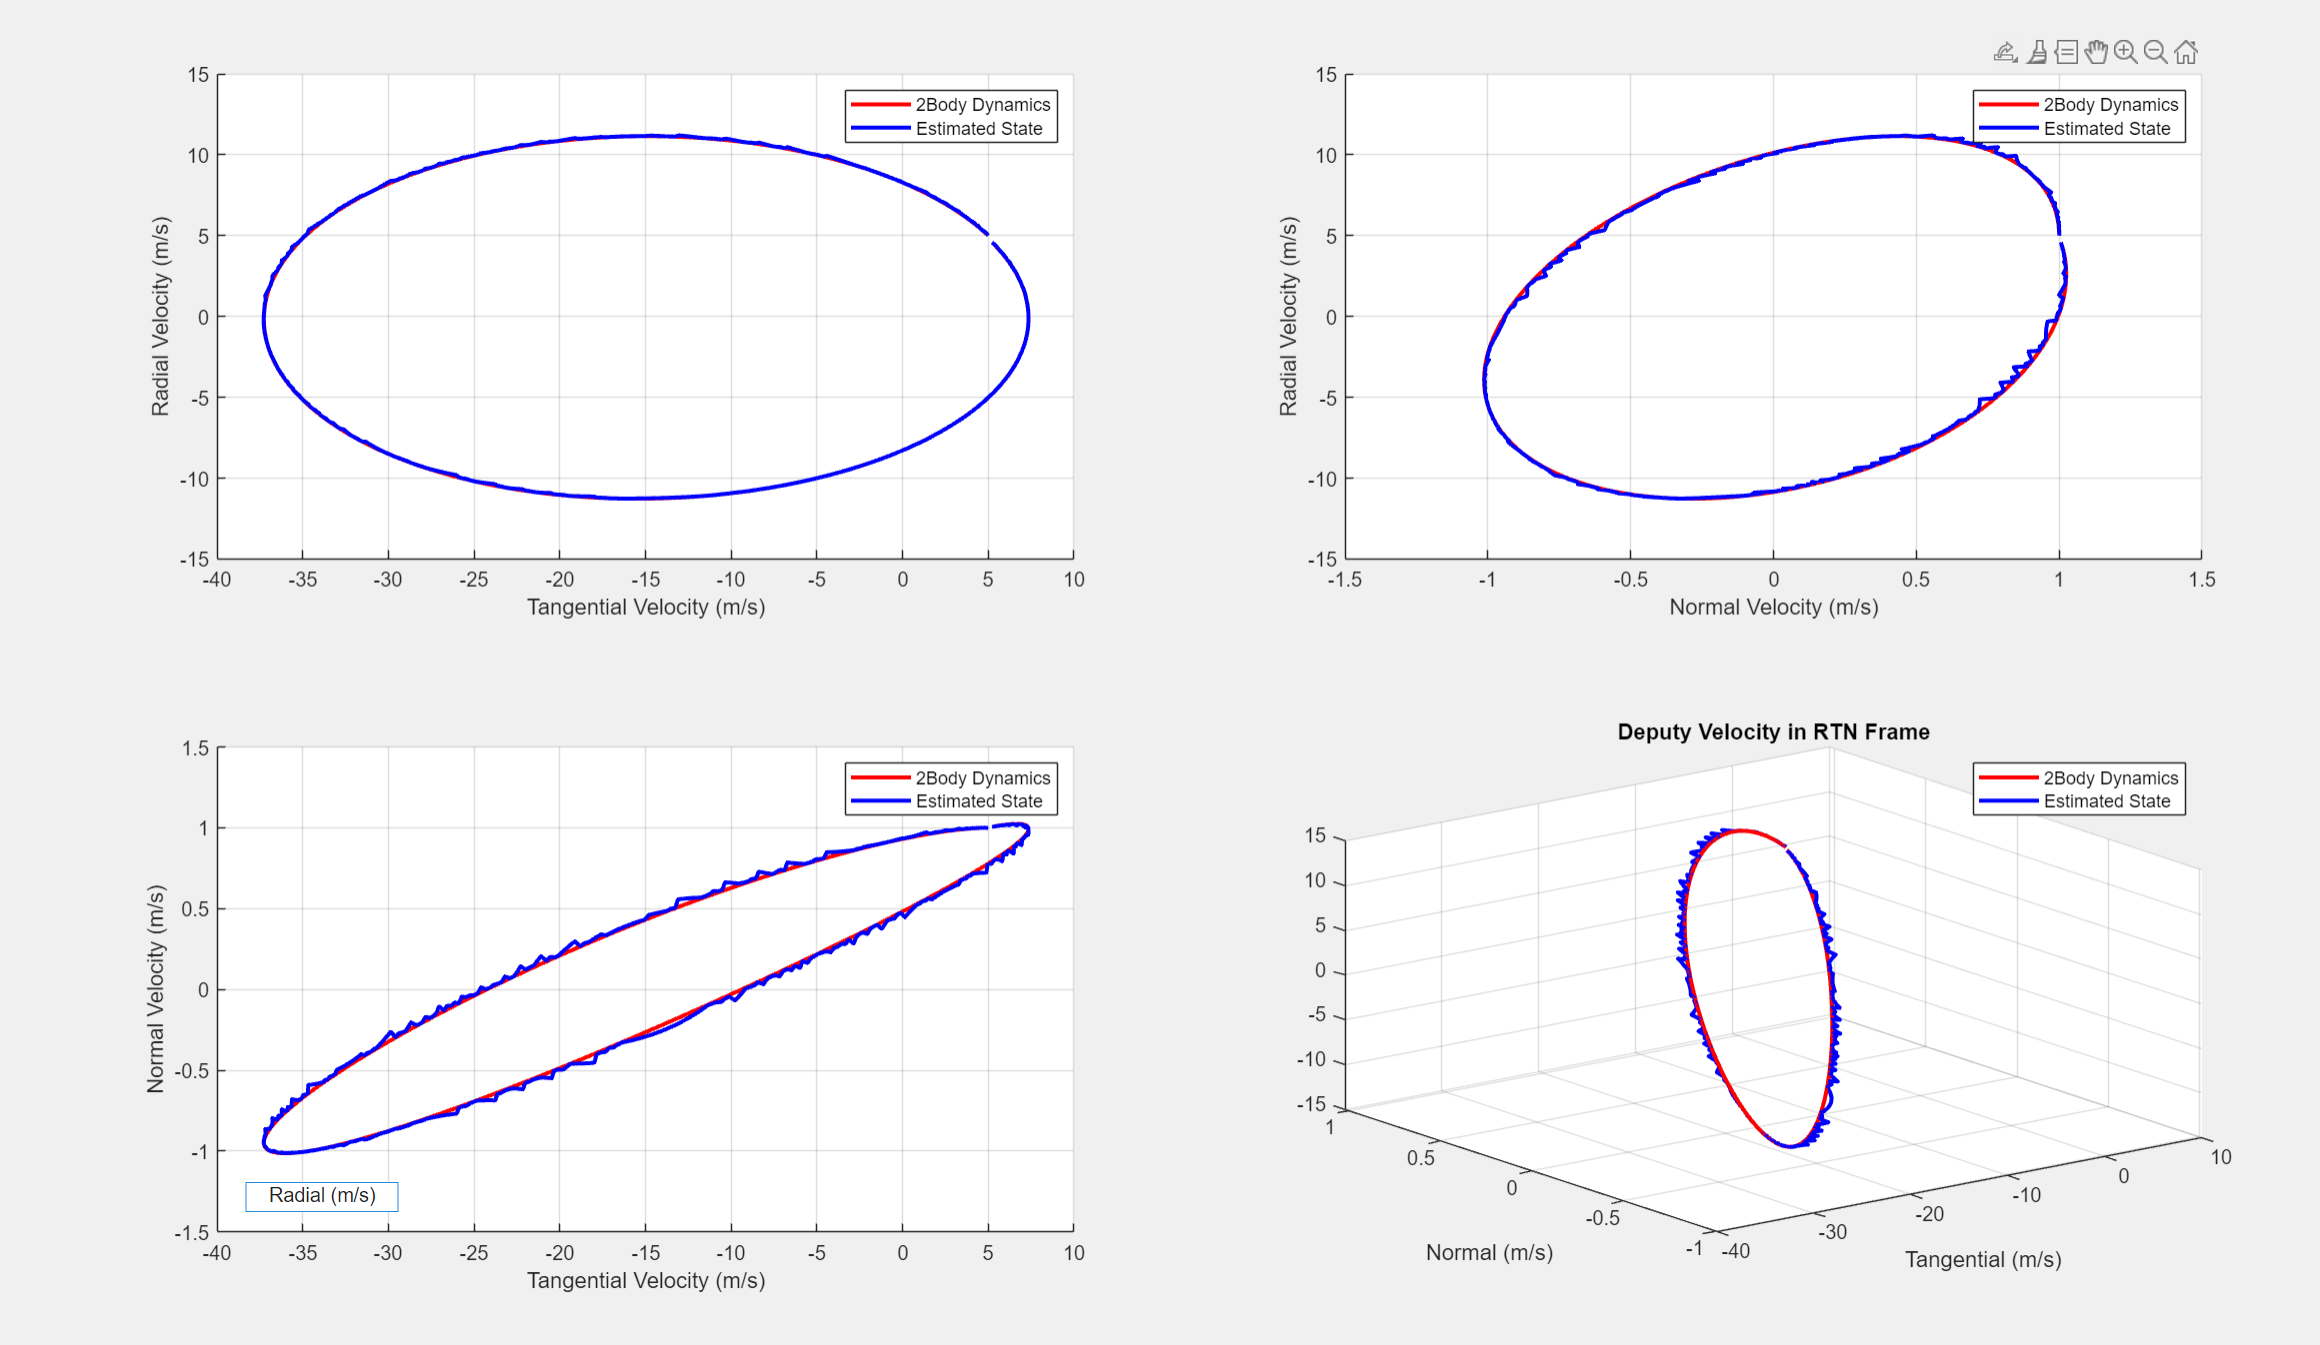
\includegraphics[width=0.7\textwidth]{PS8/Figures/velocity.png}
    \caption{Estimated Velocity}
    \label{fig:hcw_velocity}
\end{figure}

\begin{figure}[H]
    \centering
    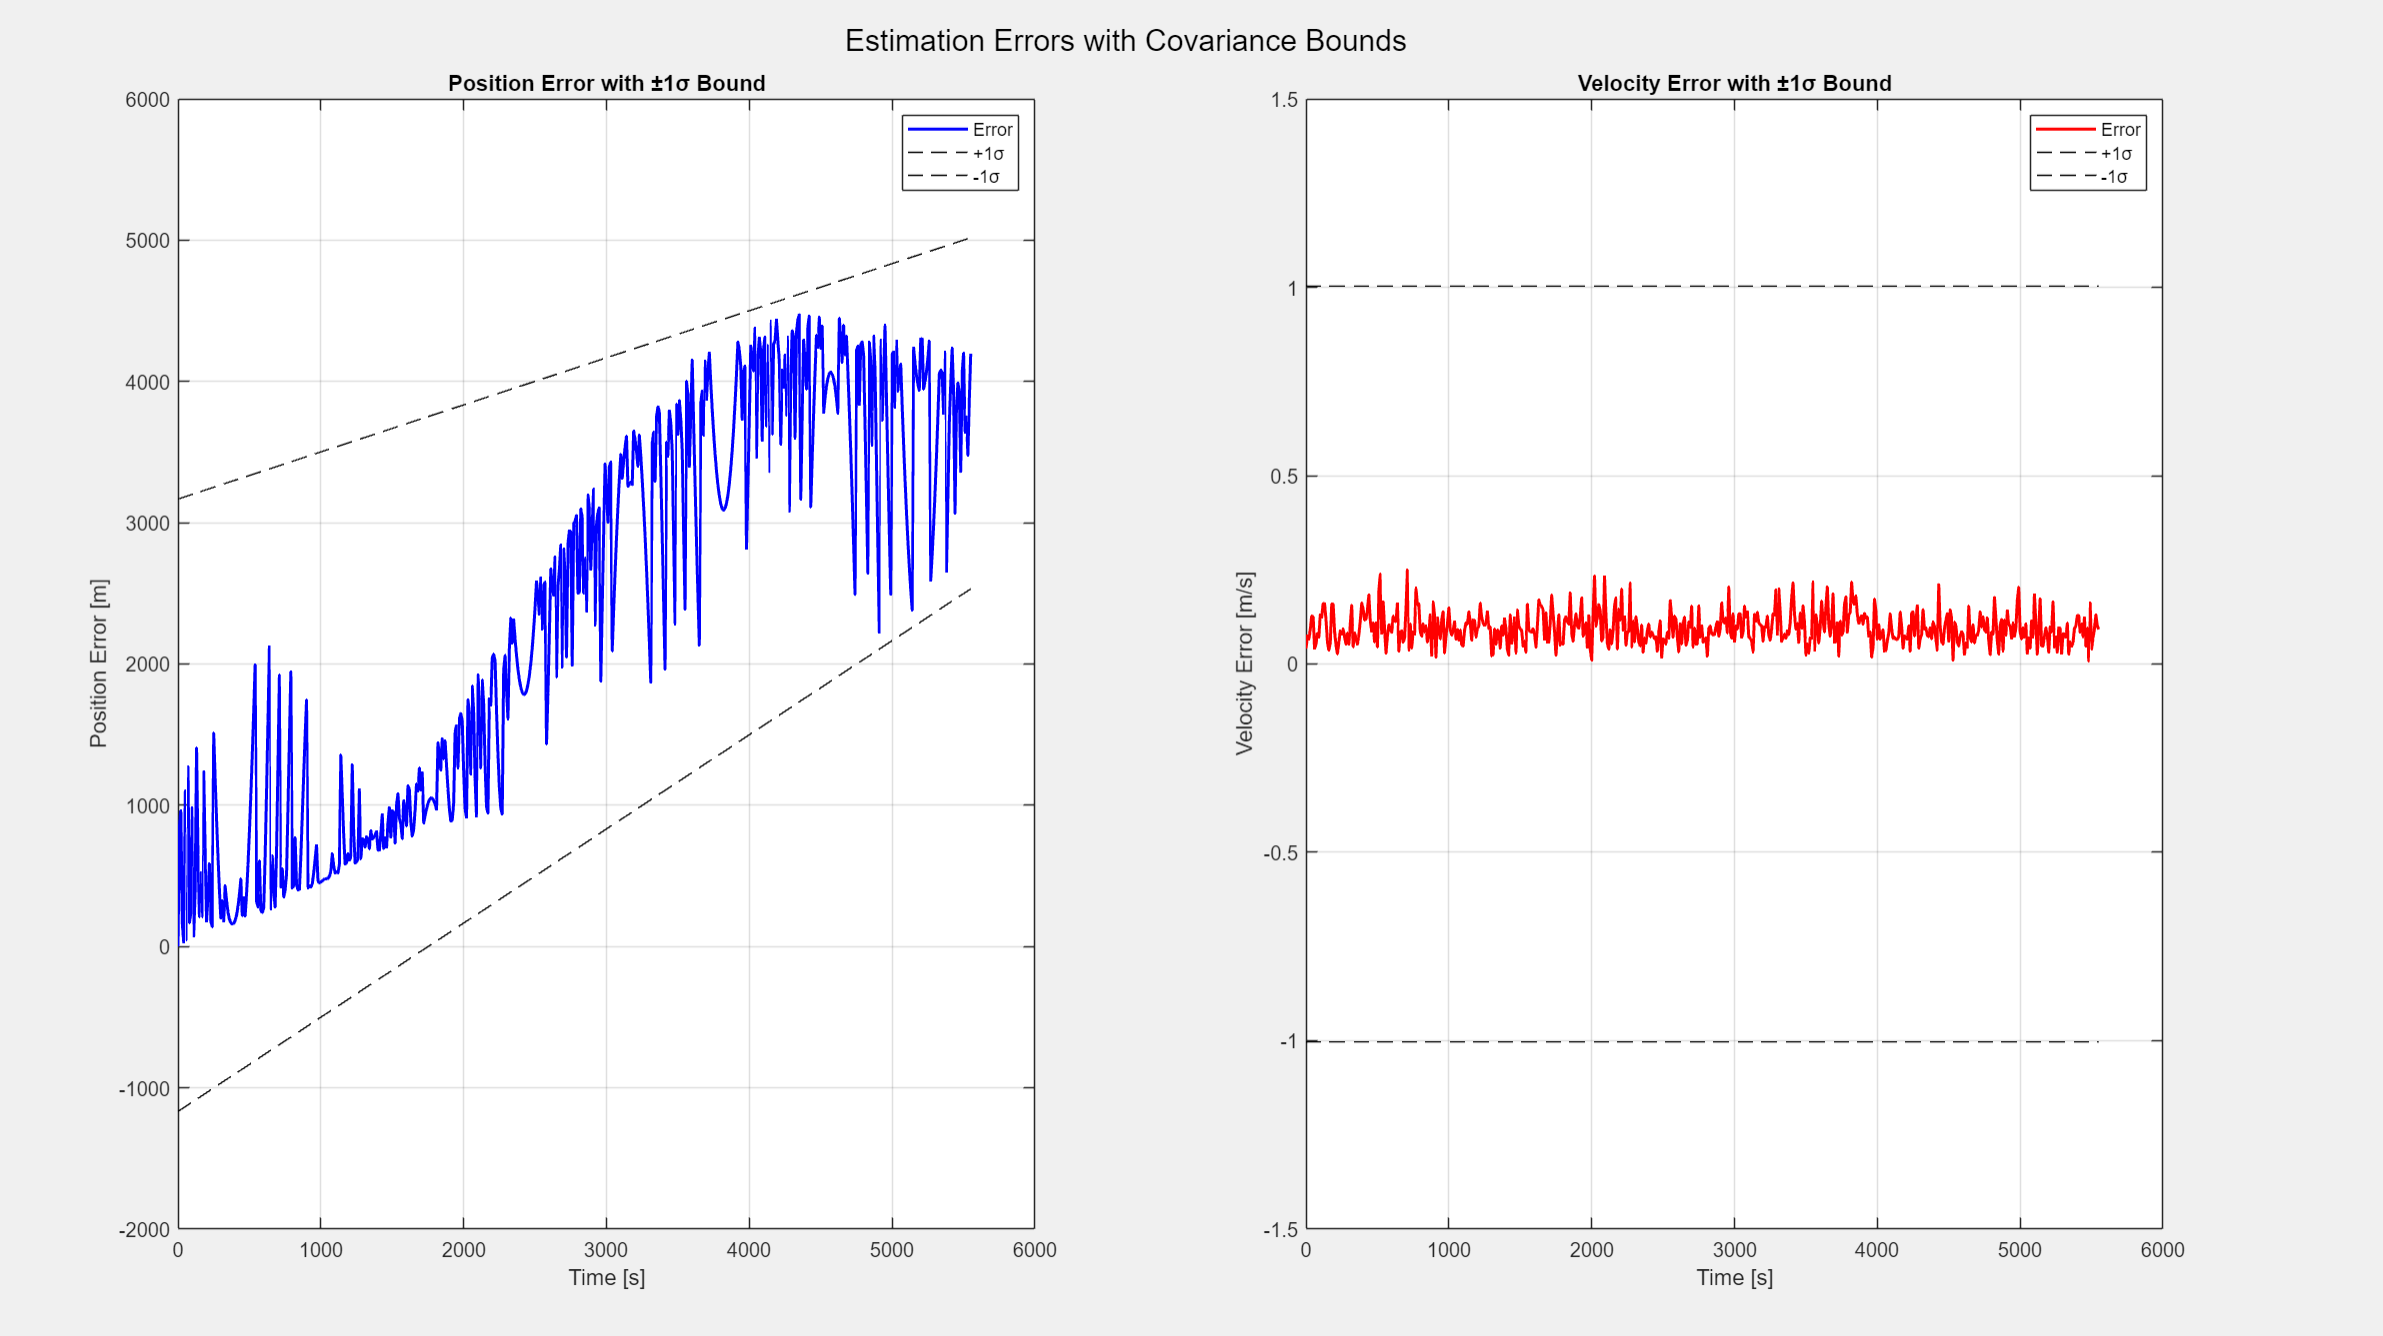
\includegraphics[width=0.7\textwidth]{PS8/Figures/error.png}
    \caption{Error in Estimate}
    \label{fig:hcw_velocity}
\end{figure}